\documentclass[12pt, notes]{beamer}
\setbeamertemplate{navigation symbols}{}

\usepackage{graphicx}
\usepackage{hyperref}
\graphicspath{ {images/} }

\title{Icaramba!\\ Iphone vulnerabilities compromise personal data}
\titlegraphic{ 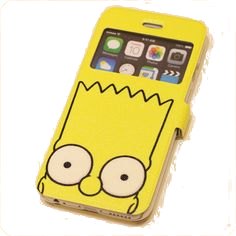
\includegraphics[width=6em]{bart_phone_case.png} }
\author{Innovatech}
\date{September 13, 2016}

\begin{document}

\begin{frame}
	\titlepage
\end{frame}

\section{Table of Contents}
\begin{frame}
	\frametitle{Table of contents}
	\tableofcontents[]
\end{frame}

\section{Initial Attack}
\begin{frame}
	\frametitle{An innocuous text}
	\begin{center}
		\begin{quote}
			New secrets about torture of Emiratis in state prisons \url{http://go.osu.edu/not_a_virus}
		\end{quote}
	\end{center}
\end{frame}
\note{An innocuous text was sent to a human rights activist from UAE. Inside there was a link that would remotely jailbreak his Iphone.\\ Since he had already been targeted before, he notified the security firm 'Citizen Lab'}

\section{How it worked}
\begin{frame}
	\frametitle{What was vulnerable?}
	\begin{center}
		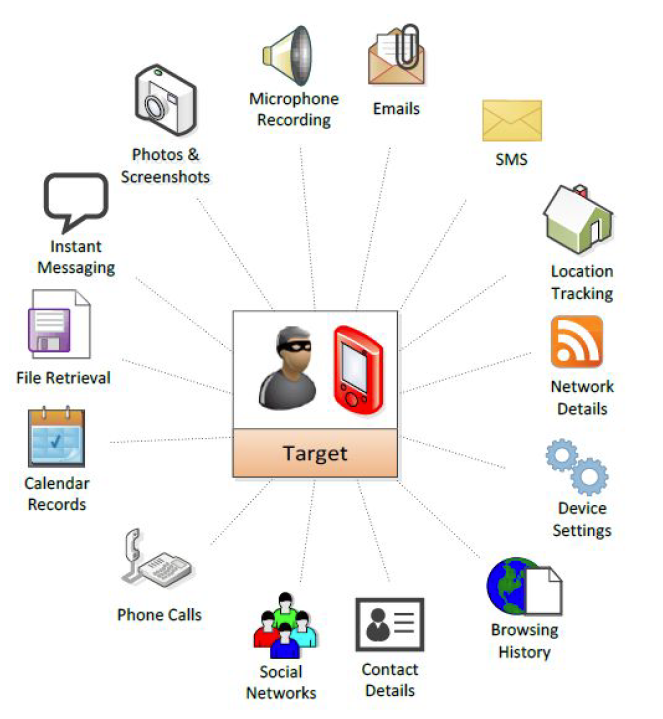
\includegraphics[height=.85\textheight]{vulnerable_data.png}
	\end{center}
\end{frame}
\note{The software was evaluated and it was determined that this link would've given access to all data accessible by the phone. It in fact incorporated three unknown vulnerabilities (also known as zero days)}

\begin{frame}
	\frametitle{Zero Day exploits}
		Zero day exploits/vulnerabilities are exploits that are unknown to a product creator, meaning there have been zero days to patch it
\end{frame}
\note{Simple explanation is simple}

\section{Who did it?}
\begin{frame}
	\frametitle{Who did it?}
		\begin{itemize}
			\item A little-known company called 'NSO Group'
			\item Based out of Tel-Aviv
			\item Sells malware to governments
		\end{itemize}
\end{frame}
\note{NSO Group was founded in 2010 and we're quoted as saying "we're a ghost". They give no interviews etc. It was only through tracing the servers it these exploits went through that the malware's codename 'Pegasus' was found. They sell malware to countries that often end up using the malware on journalists and political dissident}

\begin{frame}
	\frametitle{Malware for sale}
	
\includegraphics[width=.3\textwidth]{nso.png}
	\begin{center}
		
\includegraphics[width=.3\textwidth]{hackingteam.png}
	\end{center}
	\begin{flushright}
		
\includegraphics[width=.3\textwidth]{finfisher.png}
	\end{flushright}
\end{frame}
\note{An example of three companies that were/are in this business. Hacking team was based in Italy and had a major blunder when their servers were hacked and documents released}

\begin{frame}
	\frametitle{References}
	\textbf{Images}
	\begin{itemize}
		\item Bart Iphone case-Pinterest
		\item Diagram of vulnerable data-Motherboard(https://motherboard.vice.com/read/government-hackers-iphone-hacking-jailbreak-nso-group)
	\end{itemize}
	\textbf{Information}
	\begin{itemize}
		\item Motherboard, \href{https://motherboard.vice.com/read/government-hackers-iphone-hacking-jailbreak-nso-group}{Government Hackers Caught Using Unprecedented iPhone Spy Tool}
	\end{itemize}
\end{frame}

\end{document}
